\documentclass[a4paper, 12pt]{article}
\usepackage[utf8]{inputenc}
\usepackage{amsmath}
\usepackage{amsfonts}
\usepackage{graphicx}
\usepackage{hyperref}

\title{Apprentissage par Renforcement pour le Contrôle d'un Drone}
\author{Inès Hafassa-Maïza, Hugo Laval}
\date{\today}

\begin{document}

\maketitle

\section{Introduction}
Ce rapport décrit l'utilisation de l'apprentissage par renforcement pour contrôler un drone dans un environnement 3D avec des obstacles. Le but est de permettre au drone de naviguer de manière autonome vers une destination tout en évitant les obstacles.

\section{Formulation du Problème}
Le problème est formulé comme un processus de décision markovien (MDP) défini par l'ensemble $(S, A, P, R, \gamma)$ où :
\begin{itemize}
    \item $S$ est l'ensemble des états, représentant la position, la vitesse et la batterie du drone.
    \item $A$ est l'ensemble des actions, représentant les accélérations possibles du drone.
    \item $P$ est la fonction de transition d'état, définissant la probabilité de passer d'un état à un autre après une action.
    \item $R$ est la fonction de récompense, définissant la récompense reçue après chaque transition.
    \item $\gamma$ est le facteur de discount, représentant l'importance des récompenses futures.
\end{itemize}

L'objectif est de trouver une politique $\pi(a|s)$ qui maximise la récompense cumulée attendue :
\[
G_t = \mathbb{E} \left[ \sum_{k=0}^{\infty} \gamma^k R_{t+k+1} \mid S_t = s \right]
\]

\section{Modélisation de la Fonction de Récompense et de l'Environnement}
La fonction de récompense est un élément crucial dans l'apprentissage par renforcement, car elle guide l'agent (le drone) vers un comportement optimal. Dans notre implémentation, la fonction de récompense est conçue pour encourager le drone à atteindre sa destination tout en évitant les obstacles. Si le drone atteint sa destination, une récompense élevée de 1000 est attribuée. En revanche, une pénalité sévère de -500 est appliquée en cas de collision avec un obstacle. De plus, pour chaque mouvement, une récompense proportionnelle à la réduction de la distance par rapport à la destination est calculée, incitant le drone à se rapprocher de son objectif. Une pénalité énergétique est également appliquée pour chaque action, proportionnelle à la racine de l'accélération utilisée, afin de simuler la consommation de la batterie.

L'environnement est modélisé comme un cube tridimensionnel de taille fixe (100 unités de côté), rempli d'obstacles générés aléatoirement avec une probabilité $p$ pour chaque position dans le cube. La destination est également générée aléatoirement à chaque initialisation de l'environnement. Le drone perçoit son environnement à travers ses états internes, qui incluent sa position, sa vitesse et son niveau de batterie. Ces informations sont encapsulées dans un vecteur d'observation qui est utilisé par le modèle Actor-Critic pour prendre des décisions. Les obstacles sont perçus indirectement par le drone lorsqu'il vérifie les collisions après chaque mouvement. Cette modélisation permet de simuler un environnement réaliste et dynamique pour l'apprentissage du drone.

Les variables d'état du drone sont modélisées comme suit :
\begin{itemize}
    \item $(X)_t, (Y)_t, (Z)_t \in [0, 100]$ représentent les coordonnées de la position du drone à l'instant $t$.
    \item $(Vx)_t, (Vy)_t, (Vz)_t \in \mathbb{R}$ représentent les composantes de la vitesse du drone à l'instant $t$.
    \item $(B)_t \in [0, 1000]$ représente le niveau de batterie du drone à l'instant $t$.
\end{itemize}

Nous définissons également :
\begin{itemize}
    \item $\mathbf{X}_{\text{cible}}$ : le point de livraison.
    \item $\mathcal{O}$ : l'ensemble des obstacles.
\end{itemize}

La fonction de coût $C_t$ à minimiser est définie comme suit :
\[
C_t = -R_t = 
-1000 \cdot \mathbf{1}_{\{\mathbf{X}_t = \mathbf{X}_{\text{cible}}\}} + 500 \cdot \mathbf{1}_{\{\mathbf{X}_t \in \mathcal{O}\}} + 1000 \cdot \mathbf{1}_{\{(B)_t = 0\}} - \alpha \left\| \mathbf{X}_{t+1} - \mathbf{X}_t \right\|_2 + \beta \left\| \mathbf{A}_t \right\|_2
\]
où $\alpha$ et $\beta$ sont des coefficients de pondération pour la distance parcourue et la consommation d'énergie, respectivement, $\mathbf{X}_t = (X_t, Y_t, Z_t)$ représente la position du drone à l'instant $t$, et $\mathbf{A}_t = (Ax_t, Ay_t, Az_t)$ représente les composantes de l'accélération appliquée au drone à l'instant $t$.

\begin{figure}[h]
    \centering
    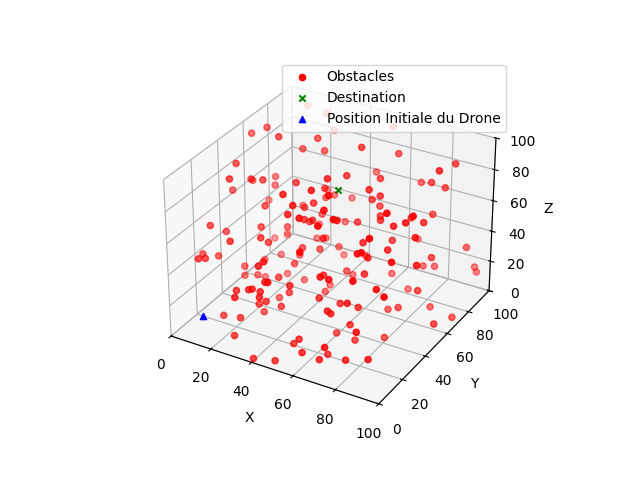
\includegraphics[width=0.8\textwidth]{Figure_1.png}
    \caption{Représentation de l'environnement 3D avec les obstacles et la destination.}
    \label{fig:environment}
\end{figure}

\section{Modèle Actor-Critic}
Le modèle Actor-Critic est utilisé pour résoudre ce problème. Il combine deux réseaux de neurones :
\begin{itemize}
    \item L'actor, qui propose des actions basées sur les états actuels.
    \item Le critic, qui évalue la qualité des actions proposées en estimant la valeur des états.
\end{itemize}

\subsection{Fonctionnement}
Le réseau Actor-Critic fonctionne en deux étapes :
\begin{enumerate}
    \item L'actor prend un état $s$ et propose une action $a$ en suivant une politique $\pi(a|s)$.
    \item Le critic évalue cette action en calculant la valeur de l'état $V(s)$ et l'avantage $A(s, a)$.
\end{enumerate}

\subsection{Fonction Objectif}
L'objectif de l'algorithme Actor-Critic est une combinaison du gradient de politique (pour l'actor) et de la fonction de valeur (pour le critic). La fonction objectif globale est généralement exprimée comme la somme de deux composants :
\begin{itemize}
    \item \textbf{Gradient de Politique (Actor)} :
    \[
    \nabla_\theta J(\theta) \approx \frac{1}{N} \sum_{i=0}^{N} \nabla_\theta \log \pi_\theta(a_i \mid s_i) \cdot A(s_i, a_i)
    \]
    où $J(\theta)$ représente le retour attendu sous la politique paramétrée par $\theta$, $\pi_\theta(a \mid s)$ est la fonction de politique, $N$ est le nombre d'expériences échantillonnées, $A(s, a)$ est la fonction d'avantage représentant l'avantage de prendre l'action $a$ dans l'état $s$, et $i$ représente l'index de l'échantillon.
    \item \textbf{Mise à Jour de la Fonction de Valeur (Critic)} :
    \[
    \nabla_w J(w) \approx \frac{1}{N} \sum_{i=1}^{N} \nabla_w (V_w(s_i) - Q_w(s_i, a_i))^2
    \]
    où $\nabla_w J(w)$ est le gradient de la fonction de perte par rapport aux paramètres du critic $w$, $V_w(s_i)$ est l'estimation du critic de la valeur de l'état $s$ avec le paramètre $w$, et $Q_w(s_i, a_i)$ est l'estimation du critic de la valeur de l'action $a$.
\end{itemize}

\subsection{Fonction d'Avantage}
La fonction d'avantage, $A(s, a)$, mesure l'avantage de prendre l'action $a$ dans l'état $s$ par rapport à la valeur attendue de l'état sous la politique actuelle :
\[
A(s, a) = Q(s, a) - V(s)
\]
où $Q(s, a)$ est la valeur de l'action et $V(s)$ est la valeur de l'état.

\section{Avantages de l'Algorithme Actor-Critic}
L'algorithme Actor-Critic offre plusieurs avantages :
\begin{itemize}
    \item \textbf{Efficacité de l'Échantillon Améliorée} : La nature hybride des algorithmes Actor-Critic conduit souvent à une meilleure efficacité de l'échantillon, nécessitant moins d'interactions avec l'environnement pour atteindre des performances optimales.
    \item \textbf{Convergence Plus Rapide} : La capacité de la méthode à mettre à jour simultanément la politique et la fonction de valeur contribue à une convergence plus rapide pendant l'entraînement, permettant une adaptation plus rapide à la tâche d'apprentissage.
    \item \textbf{Polyvalence à Travers les Espaces d'Action} : Les architectures Actor-Critic peuvent gérer de manière transparente les espaces d'action discrets et continus, offrant une flexibilité pour aborder une large gamme de problèmes d'apprentissage par renforcement.
    \item \textbf{Apprentissage Hors-Politique (dans certaines variantes)} : Apprend à partir d'expériences passées, même lorsqu'elles ne suivent pas directement la politique actuelle.
\end{itemize}

\section{Implémentation}
Le fichier \texttt{app\_renf.py} contient les classes et fonctions suivantes :
\begin{itemize}
    \item \texttt{Environment} : Génère un environnement 3D avec des obstacles et une destination.
    \item \texttt{Drone} : Représente le drone avec ses propriétés et comportements.
    \item \texttt{DroneEnv} : Interface Gym pour l'apprentissage par renforcement.
    \item \texttt{ActorCritic} : Modèle Actor-Critic pour l'apprentissage.
    \item \texttt{train} : Fonction d'entraînement pour le modèle Actor-Critic.
\end{itemize}

\section{Résultats et Discussion}
L'entraînement du modèle Actor-Critic permet au drone d'apprendre à naviguer vers la destination tout en évitant les obstacles. Les récompenses sont définies pour encourager le drone à se rapprocher de la destination et à éviter les collisions.
A COMPLETER
\section{Conclusion}
L'apprentissage par renforcement avec le modèle Actor-Critic est une approche efficace pour le contrôle autonome de drones dans des environnements complexes. Les résultats montrent que le drone peut apprendre à naviguer de manière optimale en maximisant les récompenses cumulées.
A COMPLETER
\end{document}